\chapter{Sensor design}
This chapter will cover sensor element selection, according to requirements presented previously.

Most space missions have on-board TID sensor - based od RadFET. RadFET is special type of modified p-MOSFET transistor, with well known dose dependence. In research work many COTS elements were checked for their characteristics, and they are now considered as a RadFET equivalent.

\section{Review of commercially available RadFETs}
    Commercial solutions are based on modified MOS structure (with thicker gate region). Example silicon structure is show in figure \ref{Tyndall_radfet_silicon}. Different companies produce their own RadFET devices, by designing different structure, fitted to particular requirements. Found companies produce RadFET sensor alone, leaving readout circuit design for customer. Physical phenomena for RadFET sensors is described in section \ref{Physical_phenomena_background}.

    \begin{figure}[H]
        \centering
        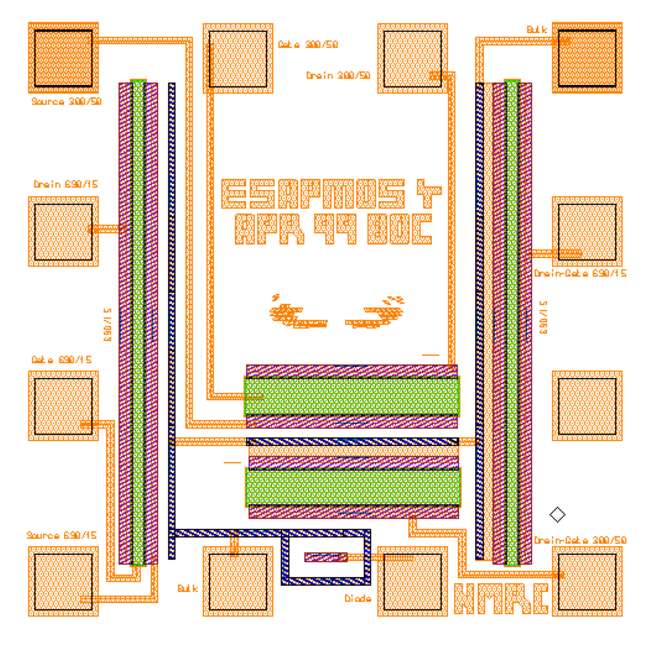
\includegraphics[width=0.5\paperwidth]{img/radfet-silicon.eps}
        \caption{4x RadFET silicon structure by Tyndall. Source: \cite{Tyndall_Radfet}}
        \label{Tyndall_radfet_silicon}
    \end{figure}


    Available products on market:

    \subsection{REM Oxford}
        REM Oxford \cite{RADFET_COM_URL}. This company produces RadFET type RFT300-CC10G1, its datasheet can be found on \cite{RFT300_CC10G1}. Structure is mounted on small carrier, as shown on figure \ref{REM_radfet_drawing}.

        \begin{figure}[H]
            \centering
            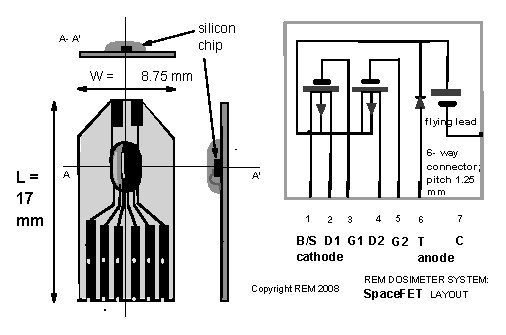
\includegraphics[width=0.5\paperwidth]{img/remOxfordDrawing.eps}
            \caption{RadFET made by REM Oxford. Source: \cite{RFT300_CC10G1}}
            \label{REM_radfet_drawing}
        \end{figure}

        This sensor consists of two PMOS transistors with modified gate structure.

        Key features:
        \begin{itemize}
            \item gate thickness \SI{200}{\nano\meter}, \SI{250}{\nano\meter} or \SI{300}{\nano\meter},
            \item sensitivity $\SI{1.5}{\milli\volt/\centi\gray} = \SI{1.5}{\milli\volt/\rad}$. Sensitivity chart is shown on figure \ref{REM_radfet_sensitivity}. At required sensitivity (\SI{1}{kRad}) threshold voltage shifts by $>\SI{100}{\milli\volt}$, depending on configuration,
            \item fading of shift is shown on figure \ref{REM_radfet_fading} - it is negligible on required mission duration ($<~\SI{3}{\percent}$),
            \item manufacturer suggests readout current in range $10-\SI{500}{\micro\ampere}$,
            \item sensor includes temperature readout from on-die diode
        \end{itemize}

        Price for one RadFET sensor begins from 800~\$.

        \begin{figure}[H]
            \centering
            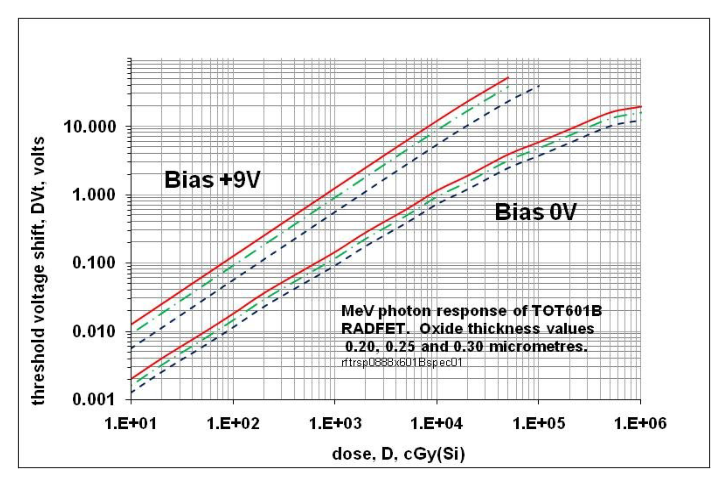
\includegraphics[width=0.6\paperwidth]{img/remSensitivity.eps}
            \caption{REM Oxford RadFET sensitivity. Source: \cite{RFT300_CC10G1}}
            \label{REM_radfet_sensitivity}
        \end{figure}

        \begin{figure}[H]
            \centering
            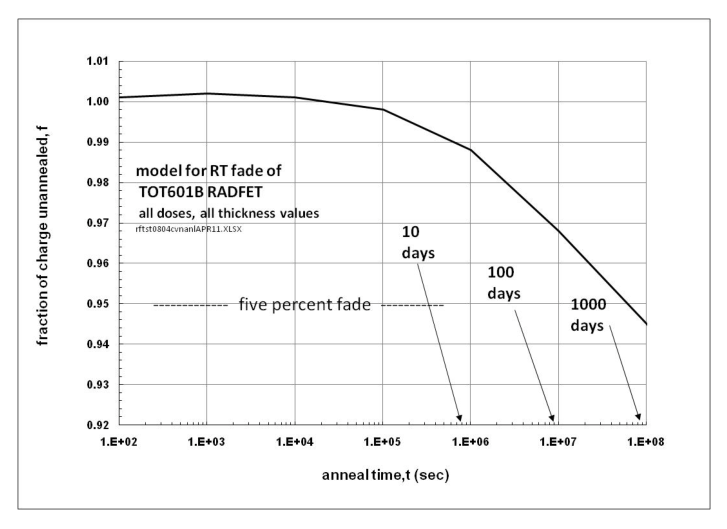
\includegraphics[width=0.6\paperwidth]{img/remOxfordFading.eps}
            \caption{REM Oxford RadFET fading. Source: \cite{RFT300_CC10G1}}
            \label{REM_radfet_fading}
        \end{figure}


    \subsection{Tyndall}
        Tyndall Works manufactures RadFET components in different packaging options \cite{TYNDALL_URL}. They provide calibration data for each type of sensor, as their response is very non-linear. Graph showing sensitivity of TY1002 is shown on figure \ref{Tyndall_TY1002_sensitivity}. Tyndall provide 4 different options, their comparison is done in table \ref{Tyndall_comparison}. Tyndall recommends grounding RadFET terminals during irradiation.

        \begin{figure}[H]
            \centering
            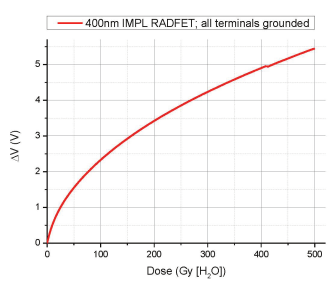
\includegraphics[width=0.6\paperwidth]{img/Tyndall_TY1002_sensitivity.png}
            \caption{Tyndall TY1002 sensitivity. Source: \cite{TYNDALL_URL}}
            \label{Tyndall_TY1002_sensitivity}
        \end{figure}

        \begin{table}[H]
        \begin{tabular}{| L{3.5cm} | C{2.5cm} | C{2.5cm} | C{2.5cm} | C{2.5cm} |}
            \hline
            Type: & TY1001 & TY1002 & TY1003 & TY1004 \\ \hline

            Image: &
            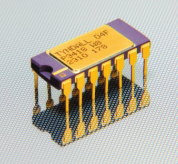
\includegraphics[width=0.12\paperwidth]{img/TY1001.png} &
            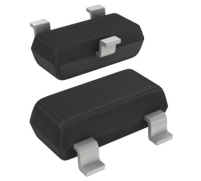
\includegraphics[width=0.12\paperwidth]{img/TY1002.png} &
            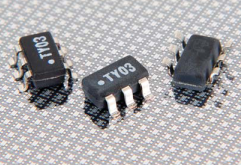
\includegraphics[width=0.12\paperwidth]{img/TY1003.png} &
            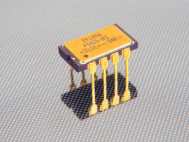
\includegraphics[width=0.12\paperwidth]{img/TY1004.png} \\ \hline

            Package: & 14-pin ceramic DILpin ceramic DIpin ceramic DI & SOT-23 & SOT23-6 & 8-pin ceramic DIL \\ \hline

            \# of transistors: & 4 & 1 & 2 & 2 \\  \hline
            W/L : & 300/50 \& 690/15 & \multicolumn{3}{c|}{300/50}  \\  \hline
            Oxide thickness: & - & - & \multicolumn{2}{c|}{\SI{400}{\nano\meter}} \\  \hline

            Maximum dose: & \multicolumn{4}{c|}{\SI{100}{\kilo\rad}} \\  \hline
            Minimal detectable dose: & \multicolumn{4}{c|}{\SI{1}{\rad}} \\  \hline

            Recommended readout current: & \multicolumn{2}{c|}{\SI{12.5}{\micro\ampere}} & \multicolumn{2}{c|}{\SI{10}{\micro\ampere}} \\ \hline

            Temperature readout: & diode & none & diode & diode \\ \hline
        \end{tabular}
        \caption{Tyndall RadFET comparison}
        \label{Tyndall_comparison}
        \end{table}


\section{COTS MOSFET as radiation sensor}
    COTS transistors parameters also depends on total dose - but in less predictable way. But this solution is much cheaper, and after self-made calibration can be considered as flight solution. According to papers, many transistors were already measured by different scientific teams. For this thesis couple of them were selected for comparison.

    P-MOSFET can have different characteristics (lower slope, higher drift and fading) than commercial RadFETs, but considering cost and space it is unfeasible for implementing RadFET-based sensor on PW-Sat2.



\section{Selected MOSFET - CD4007}

\section{Conceptual Block diagram}

    Conceptual block diagram is presented on figure \ref{conceptual_block_diagram}. It consists of mosfet, current source, analog to digital converter, die temperature sensor and interface to OBC.

    \begin{figure}[H]
        \centering
        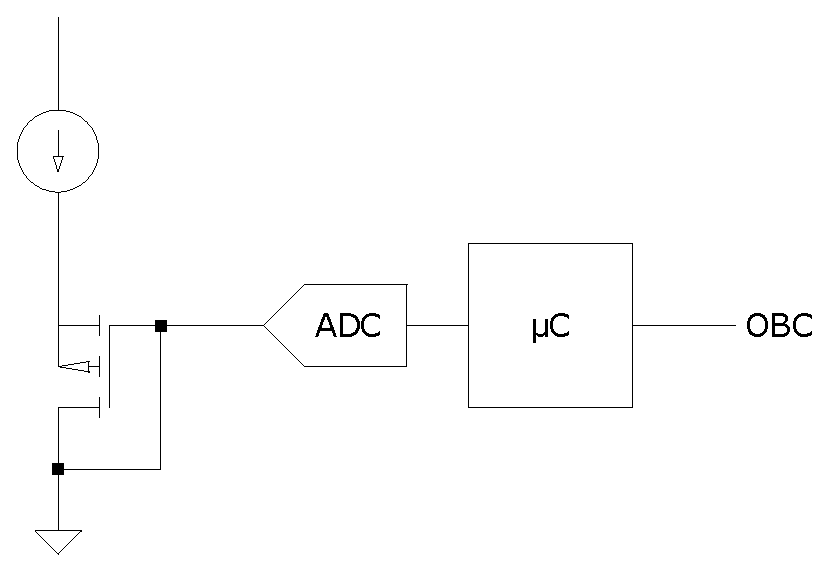
\includegraphics[width=0.3\paperwidth]{img/conceptual_block_diagram.eps}
        \caption{Threshold voltage readout block diagram}
    \end{figure}

    \subsection{Threshold voltage}
        Threshold voltage changes with TID accumulated. Easiest method to measure change of this parameter is to connect MOSFET in diode configuration, forcing constant drain current. Current source value will be selected during calibration - to achieve "zero temperature coefficient" point.

        In saturation region drain current is described by following equation (body effect is negligible):

        $$I_D = A \cdot (V_{GS} - V_{th})^2$$
        Where:

        \begin{tabular}{lcl}
            $I_D$ & - & drain current \\
            $A = \frac{\mu_n C_{ox}}{2} \frac{W}{L}$ & - & constant for partuicular transistor \\
            $V_{GS}$ & - & gate-source voltage \\
            $V_{th}$ & - & threshold voltage \\
        \end{tabular}
        \bigskip

        Because only threshold voltage change is interesting measuring $V_{GS}$ have the same effect:
        $$I_D = A \cdot (V_{GS_1} - V_{th_1})^2 = A \cdot (V_{GS_2} - V_{th_2})^2$$
        $$\Delta V_{GS} = \Delta V_{th}$$

        During irradiation current source should be disabled - as the whole sensor. This will lead to no power consumption during irradiation, enabling device only for readout.

    \subsection{Die temperature}
        Because threshold voltage strongly depends on die temperature this effect have to be compensated. Die temperature have to be measured accurately, individual MOSFET will have to be calibrated prior to launch.

        Couple of possible temperature measurement techniques were considered during this thesis:
        \begin{itemize}
            \item discrete PT-1000 sensor glued to MOSFET - this was rejected because of large heat resistance,
            \item ESD diode measurement in CD4007 - readout circuit for this solution is rather complicated, therefore it was rejected too,
            \item body diode in N-MOSFET in CD4007 package - this is chosen solution
        \end{itemize}

        The chosen solution is to measure temperature of silicon die using body diode in complementary N-MOS transistor. Thermal conductance is very high - CMOS pair is next to each other. Block diagram of proposed solution is presented on figure \ref{Temperature_measurement_block_diagram}.

        \begin{figure}[H]
            \centering
            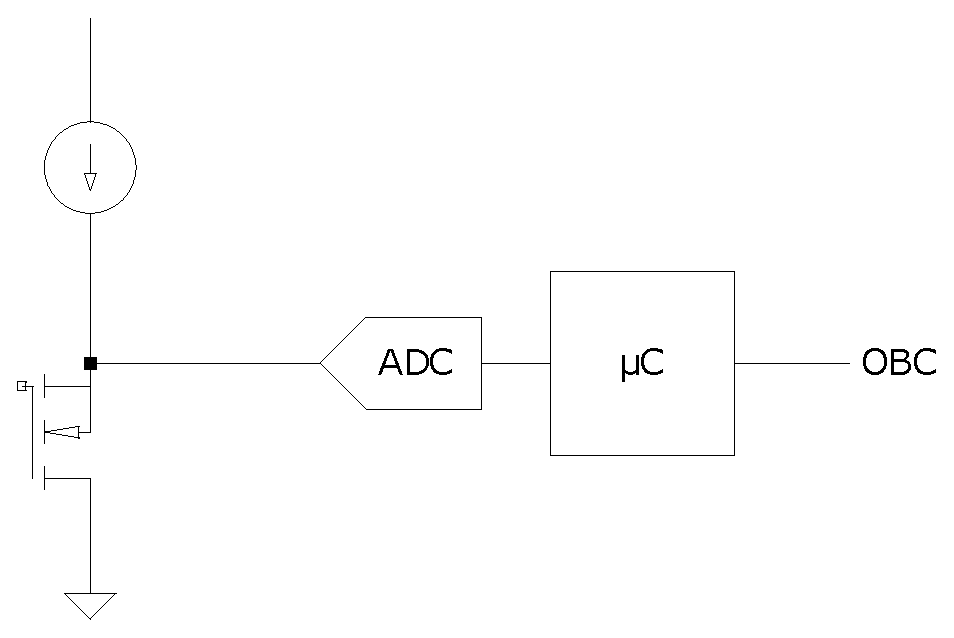
\includegraphics[width=0.3\paperwidth]{img/n-mos-temperature.eps}
            \caption{Temperature measurement block diagram}
            \label{Temperature_measurement_block_diagram}
        \end{figure}

        During calibration, temperature vs measured drop look-up table will be created. It can be used as direct conversion from read voltage to temperature, or can be approximated by function fitting.

\section{Characteristic curves (MG)}
\section{Operating point selection}
